\documentclass{homework}

\title{Homework 4}
\author{Kevin Evans}
\studentid{11571810}
\date{February 17, 2021}
\setclass{Physics}{461}
\usepackage{amssymb}
\usepackage{mathtools}

\usepackage{amsthm}
\usepackage{amsmath}
\usepackage{slashed}
\usepackage{relsize}
\usepackage{threeparttable}
\usepackage{float}
\usepackage{booktabs}
\usepackage{boldline}
\usepackage{changepage}
\usepackage{physics}
\usepackage[inter-unit-product =\cdot]{siunitx}
\usepackage{setspace}

\usepackage[makeroom]{cancel}
%\usepackage{pgfplots}

\usepackage{enumitem}
\usepackage{times}

\usepackage{amsthm}
\newtheorem*{ident}{Identity}

\renewcommand\qedsymbol{$\blacksquare$}
\usepackage{multirow}


\begin{document}
	\maketitle
	\begin{enumerate}
		\item From the frame of the electron, the proton is orbiting the electron, creating a magnetic field at the origin. With this magnetic field, the electron spin moment will have an energy $U = -\mu \cdot \bvec{B}$, with a negative sign due to the electron's charge. 
		
		\item If we take $\bvec{J}^2$ and substitute in $\bvec{L}$ and $\bvec{S}$, \begin{align*}
			\bvec{J}^2 & = \left(\bvec{L} + \bvec{S}\right)^2 \\
				& = \bvec{L}^2 + \bvec{S}^2 + 2 \bvec{L} \cdot \bvec{S} \\
			\Rightarrow \bvec{L} \cdot \bvec{S} & = \frac{1}{2} \left(\bvec{J}^2 - \bvec{L}^2 - \bvec{S}^2\right) \\
			\alpha \bvec{L} \cdot \bvec{S} & = \frac{\alpha \hbar^2}{2} \left[j(j+1) - \ell(\ell+1) - s(s+1) \right]
		\end{align*}
	
		\item It'd look something like this:
		\begin{center}
			\begin{tabular}{cc|cc|c}
				\toprule
				& $m_j$ & $m_\ell$ & $m_s$ & $m_\ell + 2 m_s$ \\
				\midrule
				\multirow{4}{*}{$j=\frac{3}{2}$} & $\frac{3}{2}$ & $1$ & $\frac{1}{2}$ & $2$ \\
					& $\frac{1}{2}$ & $0$ & $\frac{1}{2}$ & $1$ \\
					& $-\frac{1}{2}$ & $-1$ & $\frac{1}{2}$ & $0$ \\
					& $-\frac{3}{2}$ & $-1$ & $-\frac{1}{2}$ & $-2$  \\
					\midrule
				\multirow{2}{*}{$j=\frac{1}{2}$} & $\frac{1}{2}$ & $1$ & $-\frac{1}{2}$ & $0$ \\
				& $-\frac{1}{2}$ & $0$ & $-\frac{1}{2}$ & $-1$ \\
				\bottomrule
			\end{tabular}					
		\end{center}
	
		\item  For an electron with an orbital angular momentum and spin, \begin{align*}
			\bvec{\mu} = \frac{\mu}{\hbar} \left(g_\ell \bvec{L} + g_s \bvec{S}\right) &
			\intertext{But also, since $\ell$ and $s$ couple to the total angular momentum $j$, }
			\frac{\mu_B}{\hbar} \left(g_\ell \bvec{L} + g_s \bvec{S}\right) & = \frac{\mu_B}{\hbar} g_j \bvec{J} \\
			g_\ell \bvec{L} + g_s \bvec{S} & = g_j \bvec{J} \\
			g_\ell \bvec{L} \cdot \bvec{J} + g_s \bvec{S} \cdot \bvec{J} & = g_j J^2
			\intertext{And from $\bvec{L} + \bvec{S} = \bvec{J}$, we can find the dot products above in terms of $L^2$, $S^2$, and $J^2$,}
			J^2 - 2 \bvec{S} \cdot \bvec{J} + S^2 &= L^2 \\
			J^2 - 2 \bvec{L} \cdot \bvec{J} + L^2 & = S^2
			\intertext{Solving for the dot products and replacing it in the earlier equation,}
			g_\ell \frac{J^2 + L^2 - S^2}{2} + g_s \frac{J^2 + S^2 - L^2}{2} & = g_j J^2
			\intertext{Then replacing these with their expectations,}
			\frac{ g_\ell }{2} \left[ j(j+1) + \ell(\ell+1) - s(s+1) \right] &
			+ \frac{g_s}{2} \left[  j(j+1) + s(s+1) - \ell(\ell+1) \right]  = g_j j(j+1) \\
			\intertext{Solving for $g_j$,}
			g_j  = g_\ell \frac{j(j+1) + \ell(\ell+1) - s(s+1)}{2 j(j+1)} +& g_s\frac{j(j+1) + s(s+1) - \ell(\ell+1)}{2j(j+1)} 
		\end{align*}
	
		\item The Land\'e $g_j$ factor for an electron simplifies to $$g_j(j,\ell) = 1 + \frac{j(j+1) - \ell(\ell+1) + 3/4}{2j(j+1)}$$
		
		So copypastaing the table from 3 with the $g$ factor results in 
		\begin{center}
			\begin{tabular}{cccc|cc|c}
				\toprule
				& $m_j$ & $g_j$ & $g_j m_j$ & $m_\ell$ & $m_s$ & $m_\ell + 2 m_s$ \\
				\midrule
				\multirow{4}{*}{$j=\frac{3}{2}$} & $\frac{3}{2}$ & $4/3$ & $2$ & $1$ & $\frac{1}{2}$ & $2$ \\
				& $\frac{1}{2}$ & $4/3$ & $2/3$ & $0$ & $\frac{1}{2}$ & $1$ \\
				& $-\frac{1}{2}$ & $4/3$ & $-2/3$ & $-1$ & $\frac{1}{2}$ & $0$ \\
				& $-\frac{3}{2}$ & $4/3$ & $-2$ & $-1$ & $-\frac{1}{2}$ & $-2$  \\
				\midrule
				\multirow{2}{*}{$j=\frac{1}{2}$} & $\frac{1}{2}$ & $2/3$ & $1/3$ & $1$ & $-\frac{1}{2}$ & $0$ \\
				& $-\frac{1}{2}$ & $2/3$ & $-1/3$ & $0$ & $-\frac{1}{2}$ & $-1$ \\
				\bottomrule
			\end{tabular}	
		\end{center}
		
		If we compare the slopes for the weak field ($g_j m_j$) and the strong field $m_\ell + 2 m_s$, it's clear why some of the lines will have an unchanged slope and some will have to curve to match the strong field case.
		
		\item \begin{enumerate}
			\item Since the top has 3 lines and bottom has 1 line, $F=1$ and $F=0$. Then $J=I=1/2$.
			\item It'd look something like this:
			% TODO: \usepackage{graphicx} required
			\begin{center}
				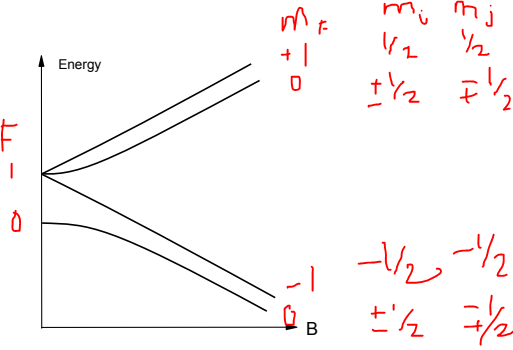
\includegraphics[width=0.7\linewidth]{hw4_6}
			\end{center}
			Although I'm a little unsure of what the $g$ factors would be and how to rank the $m_f=0$ states.
		\end{enumerate}
		
		\pagebreak
		
		\item \begin{enumerate}
			\item If $J=1/2$, then $I=3/2$ and $F=2$
			\item Maybe something like this?
			
			\begin{center}
				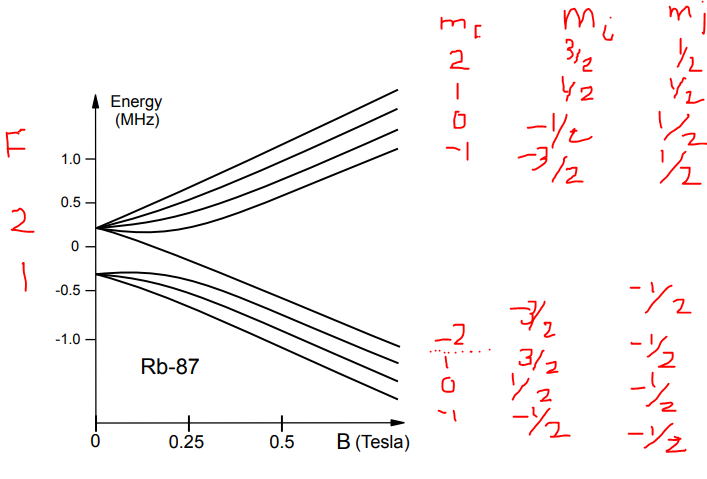
\includegraphics[width=0.7\linewidth]{hw4_7}
			\end{center}
			
		\end{enumerate}
	\end{enumerate}
\end{document}